% GENERATED by make_paper_assets.py -- do not edit by hand.
\begin{figure}[t]
\centering
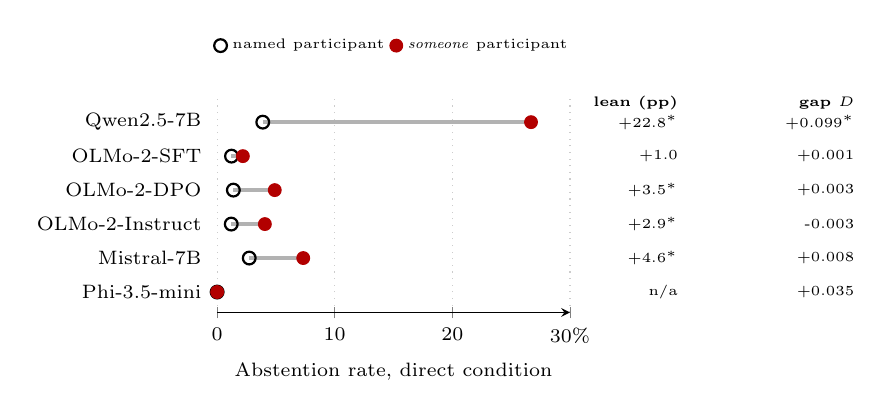
\begin{tikzpicture}
\begin{axis}[
  width=0.50\columnwidth, height=4.3cm, xmin=0, xmax=30, ymin=0.4, ymax=6.7,
  xtick={0,10,20,30}, xticklabels={0,10,20,30\%},
  ytick={6,5,4,3,2,1},
  yticklabels={Qwen2.5-7B,OLMo-2-SFT,OLMo-2-DPO,OLMo-2-Instruct,Mistral-7B,Phi-3.5-mini},
  xlabel={Abstention rate, direct condition},
  tick label style={font=\scriptsize}, label style={font=\scriptsize},
  axis lines=left, y axis line style={draw=none}, ytick style={draw=none},
  xmajorgrids, grid style={dotted, gray!40}, clip=false,
  legend style={at={(0.5,1.16)}, anchor=south, font=\tiny, draw=none, legend columns=2},
]
\draw[gray!60, line width=1.4pt] (axis cs:3.88,6) -- (axis cs:26.69,6);
\draw[gray!60, line width=1.4pt] (axis cs:1.22,5) -- (axis cs:2.19,5);
\draw[gray!60, line width=1.4pt] (axis cs:1.38,4) -- (axis cs:4.90,4);
\draw[gray!60, line width=1.4pt] (axis cs:1.20,3) -- (axis cs:4.06,3);
\draw[gray!60, line width=1.4pt] (axis cs:2.73,2) -- (axis cs:7.32,2);
\draw[gray!60, line width=1.4pt] (axis cs:0.00,1) -- (axis cs:0.00,1);
\addplot[only marks, mark=o, mark size=2.3pt, black, thick] coordinates {(3.88,6) (1.22,5) (1.38,4) (1.20,3) (2.73,2) (0.00,1)};
\addlegendentry{named participant}
\addplot[only marks, mark=*, mark size=2.3pt, red!70!black] coordinates {(26.69,6) (2.19,5) (4.90,4) (4.06,3) (7.32,2) (0.00,1)};
\addlegendentry{\textit{someone} participant}
\node[anchor=east, font=\tiny\bfseries] at (axis cs:40,6.55) {lean (pp)};
\node[anchor=east, font=\tiny\bfseries] at (axis cs:55,6.55) {gap $D$};
\node[anchor=east, font=\tiny] at (axis cs:40,6) {+22.8$^{*}$};
\node[anchor=east, font=\tiny] at (axis cs:55,6) {+0.099$^{*}$};
\node[anchor=east, font=\tiny] at (axis cs:40,5) {+1.0};
\node[anchor=east, font=\tiny] at (axis cs:55,5) {+0.001};
\node[anchor=east, font=\tiny] at (axis cs:40,4) {+3.5$^{*}$};
\node[anchor=east, font=\tiny] at (axis cs:55,4) {+0.003};
\node[anchor=east, font=\tiny] at (axis cs:40,3) {+2.9$^{*}$};
\node[anchor=east, font=\tiny] at (axis cs:55,3) {-0.003};
\node[anchor=east, font=\tiny] at (axis cs:40,2) {+4.6$^{*}$};
\node[anchor=east, font=\tiny] at (axis cs:55,2) {+0.008};
\node[anchor=east, font=\tiny] at (axis cs:40,1) {n/a};
\node[anchor=east, font=\tiny] at (axis cs:55,1) {+0.035};
\end{axis}
\end{tikzpicture}
\caption{Abstention concentrates on unnamed participants in every checkpoint that
abstains, but only Qwen2.5 abstains enough for it to matter downstream.
Each row joins the abstention rate on named-participant items (open) to that on
\textit{someone} items (filled). \emph{Lean} is the difference in percentage points, and
$D$ is the resulting gap in ground-truth recovery error (Sec.~\ref{sec:models}).
$^*$: significant after Holm correction across the five abstaining checkpoints
(lean) or permutation $p<0.05$ ($D$). Phi-3.5-mini never abstains
(0 of 7{,}680 draws).}
\label{fig:abstention}
\end{figure}
